%
%
%

\chapter{Introduction to Control Engineering with Python}

\section{Problem Statement and Learning Objectives}

This brief chapter will introduce
some control engineering computations with Python.  After completing this
chapter the student should be able to
\begin{itemize}
    \item Apply previous knowledge of Python basics to numerical evaluation of problems in this
    course.   We will use
    \begin{itemize}
            \item numpy, scipy, and matplotlib packages (python control references a package called Slycot but we do not need it.)
            \item python 3 (3.12 or later)  (command line or notebook environments)
            \item package python control (version 0.10+)
    \end{itemize}
    \item Write or adapt python scripts for control related computations including:
    \begin{itemize}
        \item enter a transfer function.
        \item Generate Bode and Root Locus Plots
        \item Correct the axis scales on plots to increase quality and readability of
        graphics plots.
        \item Use and adapt a supplied python package to optimize gains for PID control
        design in spite of actuator saturation and other non-ideal factors.
    \end{itemize}
\end{itemize}



\section{Links and details}
For download and detailed documentation, please see

\href{python control}{https://pypi.org/project/control/}

\href{Install Python on Windows}{https://learn.microsoft.com/en-us/windows/python/beginners}


\section{Root Locus Example with AI}

First, let's try the Root locus plot of Example 6.8 again with help from {\tt Claude.ai}.
The open loop gain is:

\beq\label{pythonRLsystem}
G(s) = C(s)P(s) = \frac {K(s+4)(s+5)} {(s+1+3j)(s+1-3j)}
\eeq


\begin{listing}
    \begin{minted}{python}
import numpy as np
import control
import matplotlib.pyplot as plt

# Define the numerator and denominator coefficients
# For numerator: K(s+4)(s+5) = Ks^2 + 9Ks + 20K
# For denominator: (s+1+3j)(s+1-3j) = s^2 + 2s + 10
num = [1, 9, 20]  # Coefficients for s^2 + 9s + 20 (K will be added by rlocus)
den = [1, 2, 10]  # Coefficients for s^2 + 2s + 10

# Create the transfer function
sys = control.TransferFunction(num, den)

# Create the root locus plot
plt.figure(figsize=(10, 8))
control.root_locus(sys, grid=True)

# Add title and labels
plt.title('Root Locus Plot')
plt.xlabel('Real Axis')
plt.ylabel('Imaginary Axis')

# Customize the grid
plt.grid(True, linestyle='--', alpha=0.7)

# Add annotations for poles and zeros
plt.plot([-4], [0], 'o', markersize=10, label='Zeros')  # Zero at s=-4
plt.plot([-5], [0], 'o', markersize=10)  # Zero at s=-5
plt.plot([-1], [3], 'x', markersize=10, label='Poles')  # Pole at s=-1+3j
plt.plot([-1], [-3], 'x', markersize=10)  # Pole at s=-1-3j

plt.legend()
plt.show()
    \end{minted}
    \caption{Root Locus plotting (and annotation) code generated by Claude.ai.}
    \label{lst:RLGenByAI}
\end{listing}


An example was simply generated by asking Claude.ai to plot the root locus of the above loop gain (input to Claude as LaTex code). The prompt is:
\begin{verbatim}

    please use python.control to plot the root locus diagram for the following loop gain:
    G(s) = C(s)P(s) = \frac {K(s+4)(s+5)} {(s+1+3j)(s+1-3j)}
\end{verbatim}

The result is given in Listing \ref{lst:RLGenByAI}.
Note that LaTex code was used to describe the transfer function and Claude.ai figured it out.

% 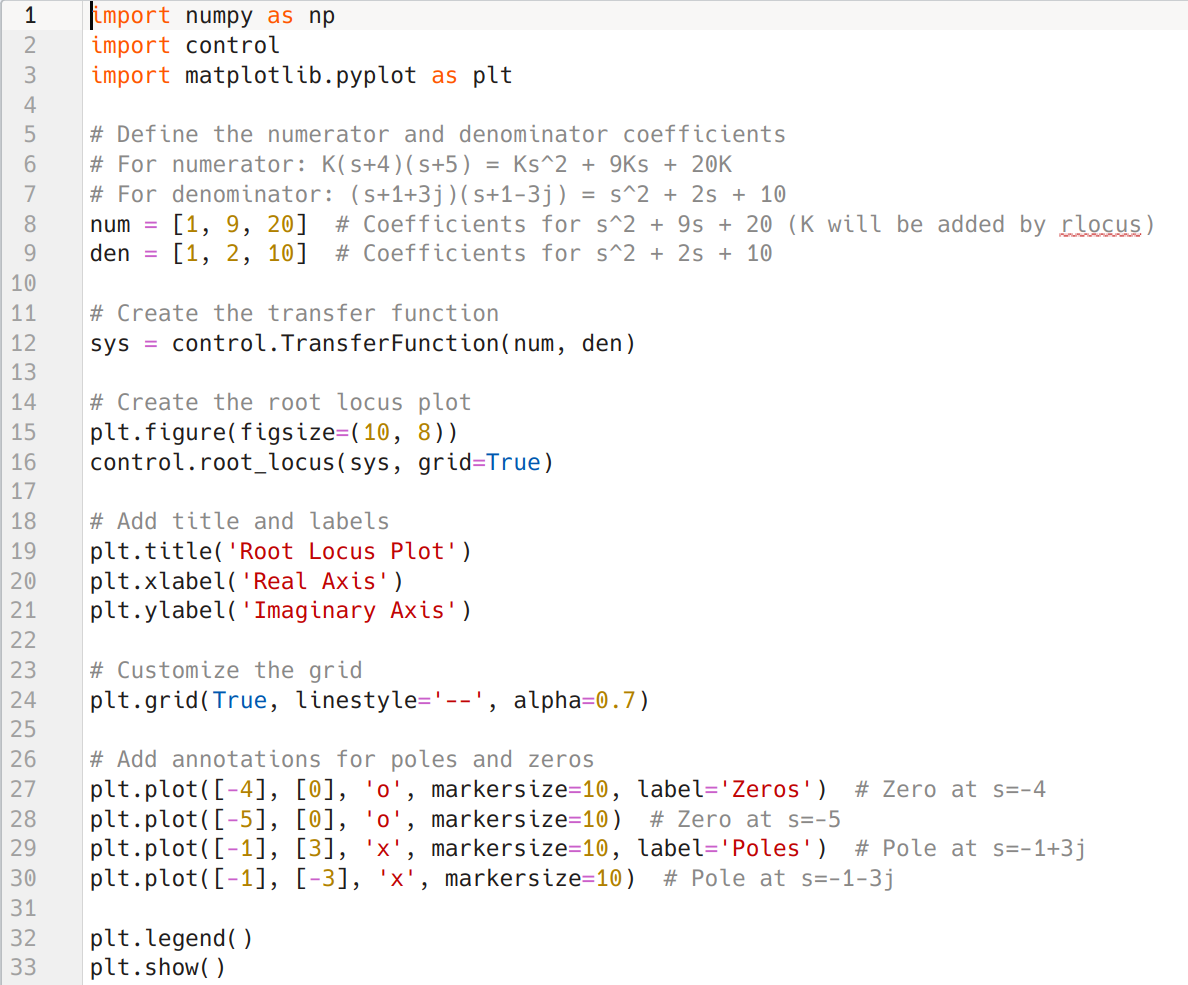
\includegraphics[width=0.6\textwidth]{figs08/B29H90.png}
In lines 8,9 the poles and zeros given as vectors of the coefficients of the powers of $s$.
Note how Claude explained their
derivation in comments! (lines 5-7).  For example in the
numerator:
\[
(s+4)(s+5) = s^2 + 9s + 20 \to [1, 9, 20]
\]
Then in line 12,
we use the {\tt control.TransferFunction(num, den)}  call to make the numerator and denominator into
a {\tt TransferFunction()} object (line 11).

Then in lines 15 and 16, we open a figure in {\tt matplotlib} and use the {control.root\_locus()} method to plot it.


Claude has added some nice features to the plot (Figure \ref{pythonRLoutput})
such as using polar coordinates
for the axes (we'll see a neat use for that later).   Also, it has done a nice job
{\bf equalizing} the axis ranges so that 1 unit on the real axis is the same number
    of image pixels as 1 unit on the imaginary axis.  This gives us insights we can
    take from the pole locations.

The AI frontier is rapidly evolving.  Who knows how many control engineering problems it will soon be able
to reliably solve.  BUT, right now results can be unreliable you really need to be able to check the correctness
of AI generated results - they are not (yet?) a substitute for understanding the underlying methods.

%
% \section{Plotting Ranges for high quality graphics}
% Sometimes autoranges provided by graphing software do not result in a graph which shows the desired features.
%
% The default ranges this time are OK but it feels like integer value axis limits would look better
% so those are explicitly set in lines 21,22.
%
% This is more important when you plot and compare multiple different root loci.   With autoranging,
% all the plots can look the same until you read the axis limits which defeats the purpose of plotting.


\begin{figure}[b]
    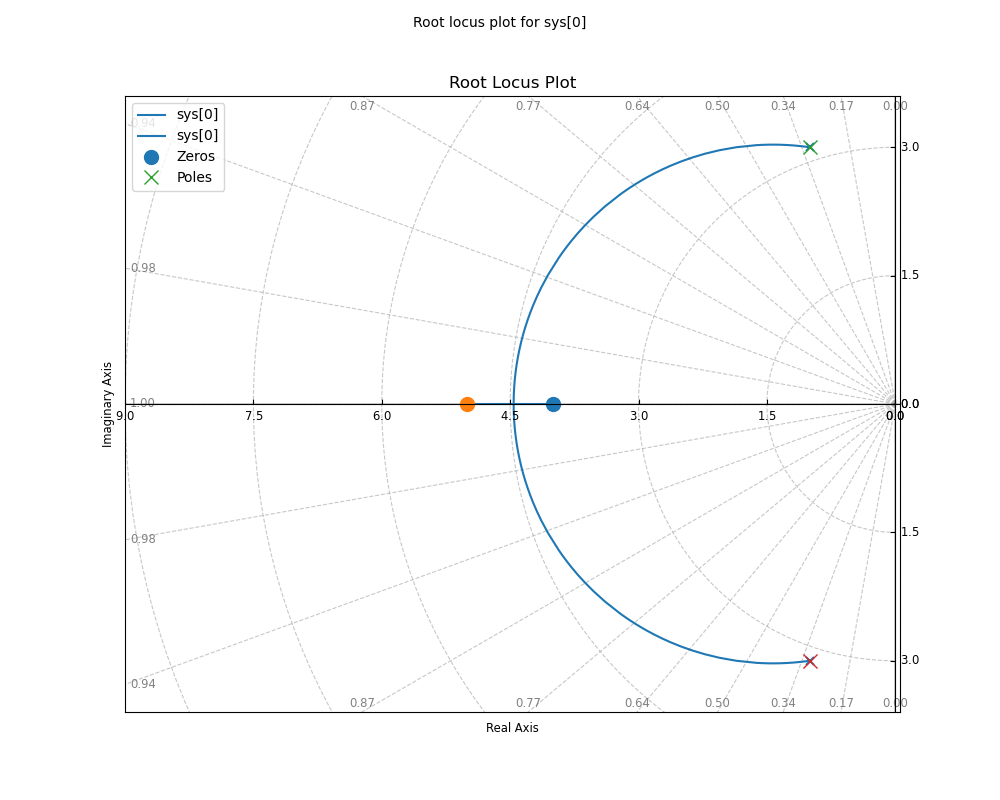
\includegraphics[width=\textwidth]{figs08/B31H79.png}
    \caption{Root locus of the system of Equation \ref{pythonRLsystem}.}\label{pythonRLoutput}
\end{figure}

\clearpage
\section{Summary of System Setup in Python}
{\tt python.control} supports three ways that you can create a ctl.LTI object (LTI = ``Linear Time Invariant").

\subsubsection{1.) Polynomial Vectors}
Here, {\tt python.control} requires multiplying out zeros and  poles and encoding
the resuling polynomials as vectors such as
\[
s^3 + 37s^2 + 123.4s + 259.5 \quad \to \quad [1, 37, 123.4, 259.5]
\]
Not too hard.  Once this is done we give them to python directly e.g.

\begin{verbatim}
    num = [1 5]
    den = [1,37,123.4,259.5]
    syst = ctl.TransferFunction(num,den) # note two separate parameters
\end{verbatim}

\subsubsection{2.) The ``$s$ is a transfer function" Trick}
Python control transfer function objects are quite smart and they can be added,
subtracted, multiplied, and divided with each other and with constants.
Plain old $s$ could be a transfer function so in fact we can build up interesing
transfer functions using it as follows:
\begin{verbatim}
    s = ctl.TransferFunction.s   # official way to create LaPlace 's'
    num = 1.0E5*(s+20)
    den = (s+500)*(s+3000)*(s*s + 4*s + 32)
    system = num/den   # note use of division for numerator and demoniator
\end{verbatim}
Since $s$ is already a {\tt ctl.TransferFunction()}  (from the first line), then
the variable {\tt system} is as well(!)

\subsubsection{3.) The State Space method}
The basic state space model from Chapter 4 is


\[
\dot{X} = AX+BU
\]
\[
\dot{X} = \begin{bmatrix}\dot{x} \\ \ddot{x} \end{bmatrix} \quad
x = \begin{bmatrix} x \\ \dot{x}  \end{bmatrix}
\]
\[
Y = CX+DU
\]
The matrices $A,B$ determine how the state evolves from inputs $U$, and
the matrices $C,D$ determine how outputs are generated (if they are not
already given by the state variables which can sometimes happen).

Let's say we have a 2 dimensional state vector $X=[x,\dot{x}]^T$ and
a single input, $f(t)/M$. The way this needs to be set up for state
space is
\[
\dot{X} = AX + [0,1/M]\begin{bmatrix} 0 \\f(t) \end{bmatrix}
\]

or in more detail
\[
\begin{bmatrix}\dot{x}\\ \ddot{x}\end{bmatrix} = A\begin{bmatrix}x\\ \dot{x}\end{bmatrix} + [0,1]\begin{bmatrix} 0\\u \end{bmatrix}
\]
other words, our input matrix
\[
B = [0,1/M]
\]
which is a row vector or a 1x2 matrix.

{\tt python.control} relies on {numpy} for matrix algebra but that is
slightly finicky when it comes to 1 dimensional matrices, i.e. vectors.
Thinking mathematically we could write
\[
x = a^T
\]
where
\[ a = [1, 2, 3] \;, x = \begin{bmatrix} 1\\2\\3 \end{bmatrix}
\]
and be fine with it.   Numpy needs vectors to be ``two-dimensional" so that it
can tell the difference between row vectors and column vectors.

Here are some quick helper functions to always initialize vectors with your
row/column intention:
\begin{verbatim}
    def RowVector(x):  # vectors in numpy have to be 2-dimensional(!)
        x = np.array(x)
        return np.atleast_2d(x)

    def ColVector(x):
        return RowVector(x).T
\end{verbatim}




\begin{ExampleSmall}
    Let's review the small SS system from Section \ref{SecSystemMatricesFromEOMs}.
    \[
    \dot{X} =
    \begin{bmatrix}\dot{x} \\ \ddot{x} \end{bmatrix} =
    \begin{bmatrix}0&1\\\frac{-(K_1+K_2)}{M}&\frac{-B}{M}\end{bmatrix}
    \begin{bmatrix}x\\ \dot{x}\end{bmatrix}+
    \begin{bmatrix}0&\frac{1}{M}\end{bmatrix}
    \begin{bmatrix}0\\f(t)\end{bmatrix}
    \]

{\bf Problem: }  Input the above state space system into {\tt python.control}
by deriving $A,B,C,D$ using the
ctl.ss(A,B,C,D) method
and compute step response. Also make a phase plot.   Assume the following
values for input and system parameters:
\[
    K1 = 10.0\\
    K2 = 20.0\\
    B = 10.0\\
    M = 100.0\\
    f(t) = 5u(t)
\]
The states of our system are inside some kind of opaque box such that the output
we can actually measure
is $y = 2x+0.7\dot{x}$.   Design the
matrices C and D.

\noindent
{\bf Solution:}

Referring to Listing \ref{lst:4x4ssSetup}:

% 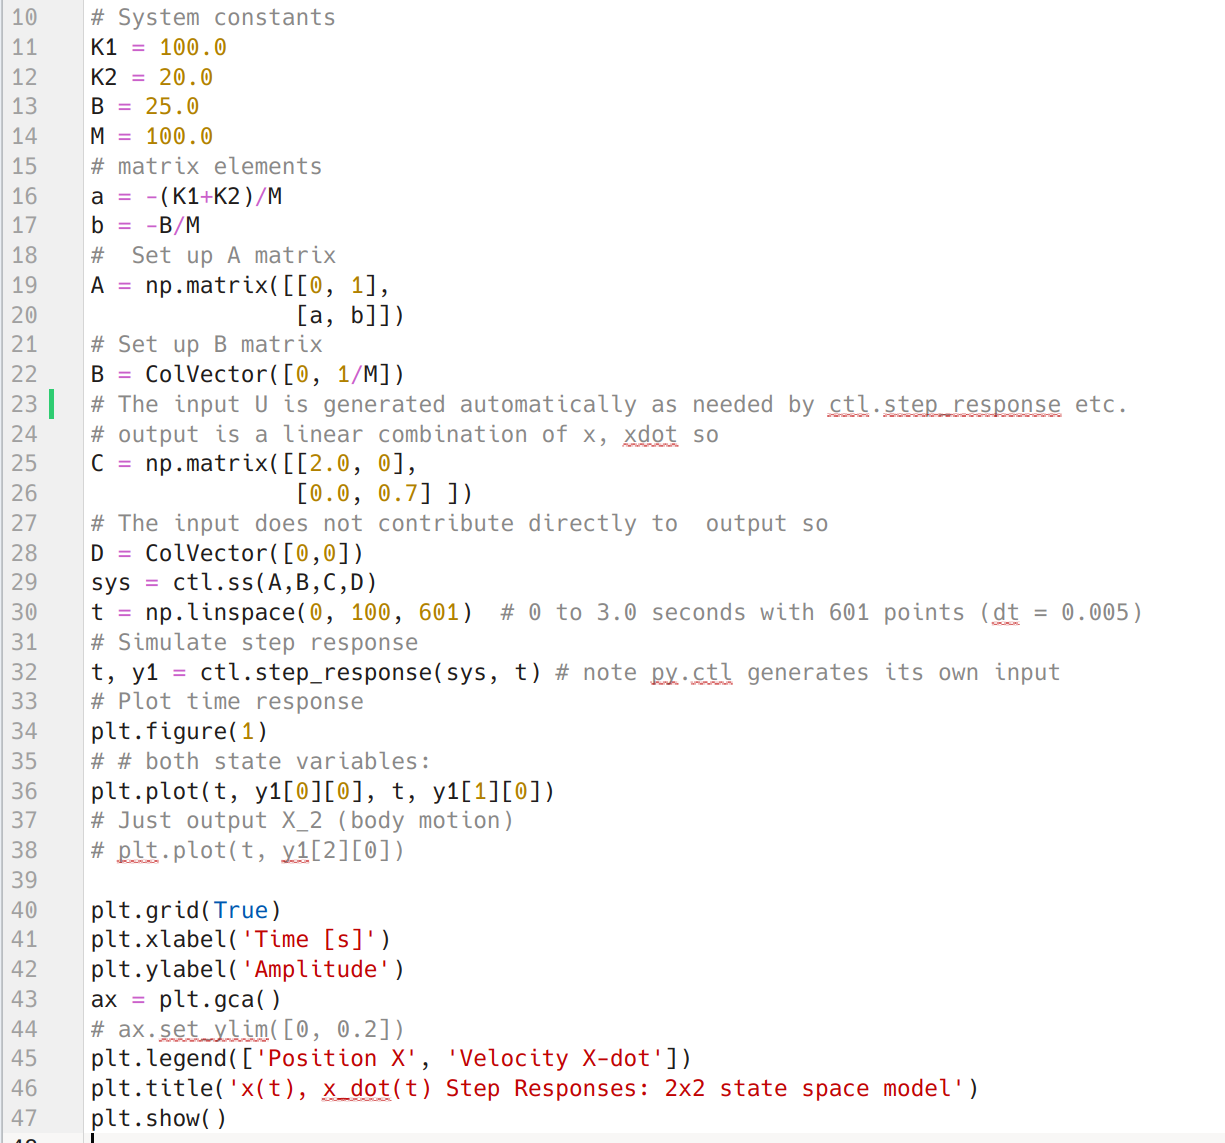
\includegraphics[width=0.5\textwidth]{figs08/B14H53.png}
In lines 10-22 we define the EOM terms and set up $A$ and $B$ matrices.

We have this unusual output in which the output is a linear combination
of the states which we implement with the $C$ matrix.
Note that for this single output case, $C$ could be 2x2 or a 2x1 column vector
equivalently:
\[
C = \begin{bmatrix} 2 \\ 0.7 \end{bmatrix}
\]


Finally,
there is no contribution of input {\tt directly} to the output, so
\[
D= \begin{bmatrix} 0,&0\\0,&0 \end{bmatrix}
\]


Performing step response
{\bf ************  To be completed}


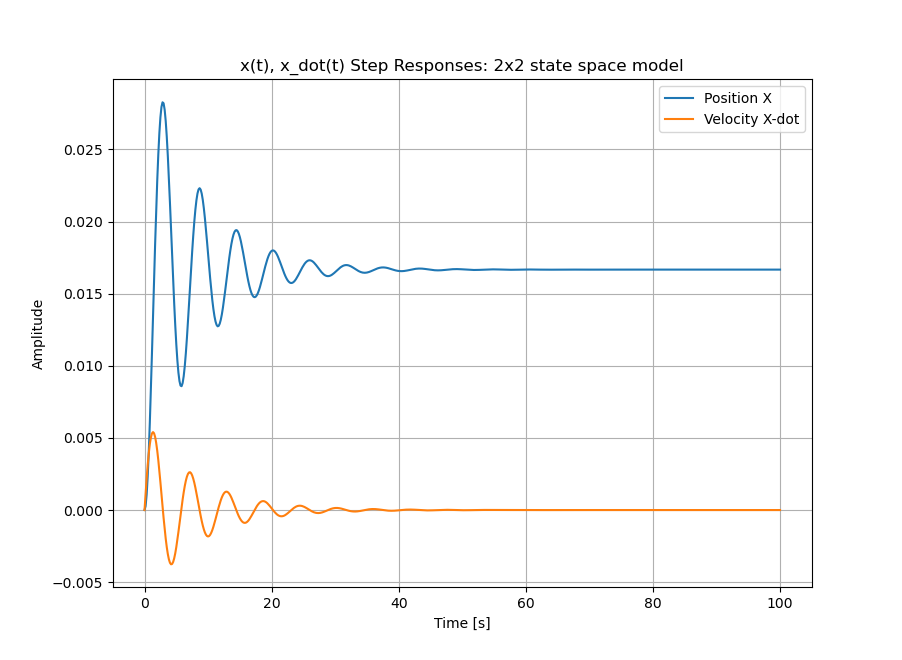
\includegraphics[width=0.5\textwidth]{figs08/B14H54.png}
\end{ExampleSmall}
% \section{Summary of Notation}



\begin{Example}
4x4 State space example in python.

The  python code in Listing \ref{lst:ss4x4} sets up the state equations for
Example  4.\ref{suspensionstatespace}.
%
% \begin{center}
%     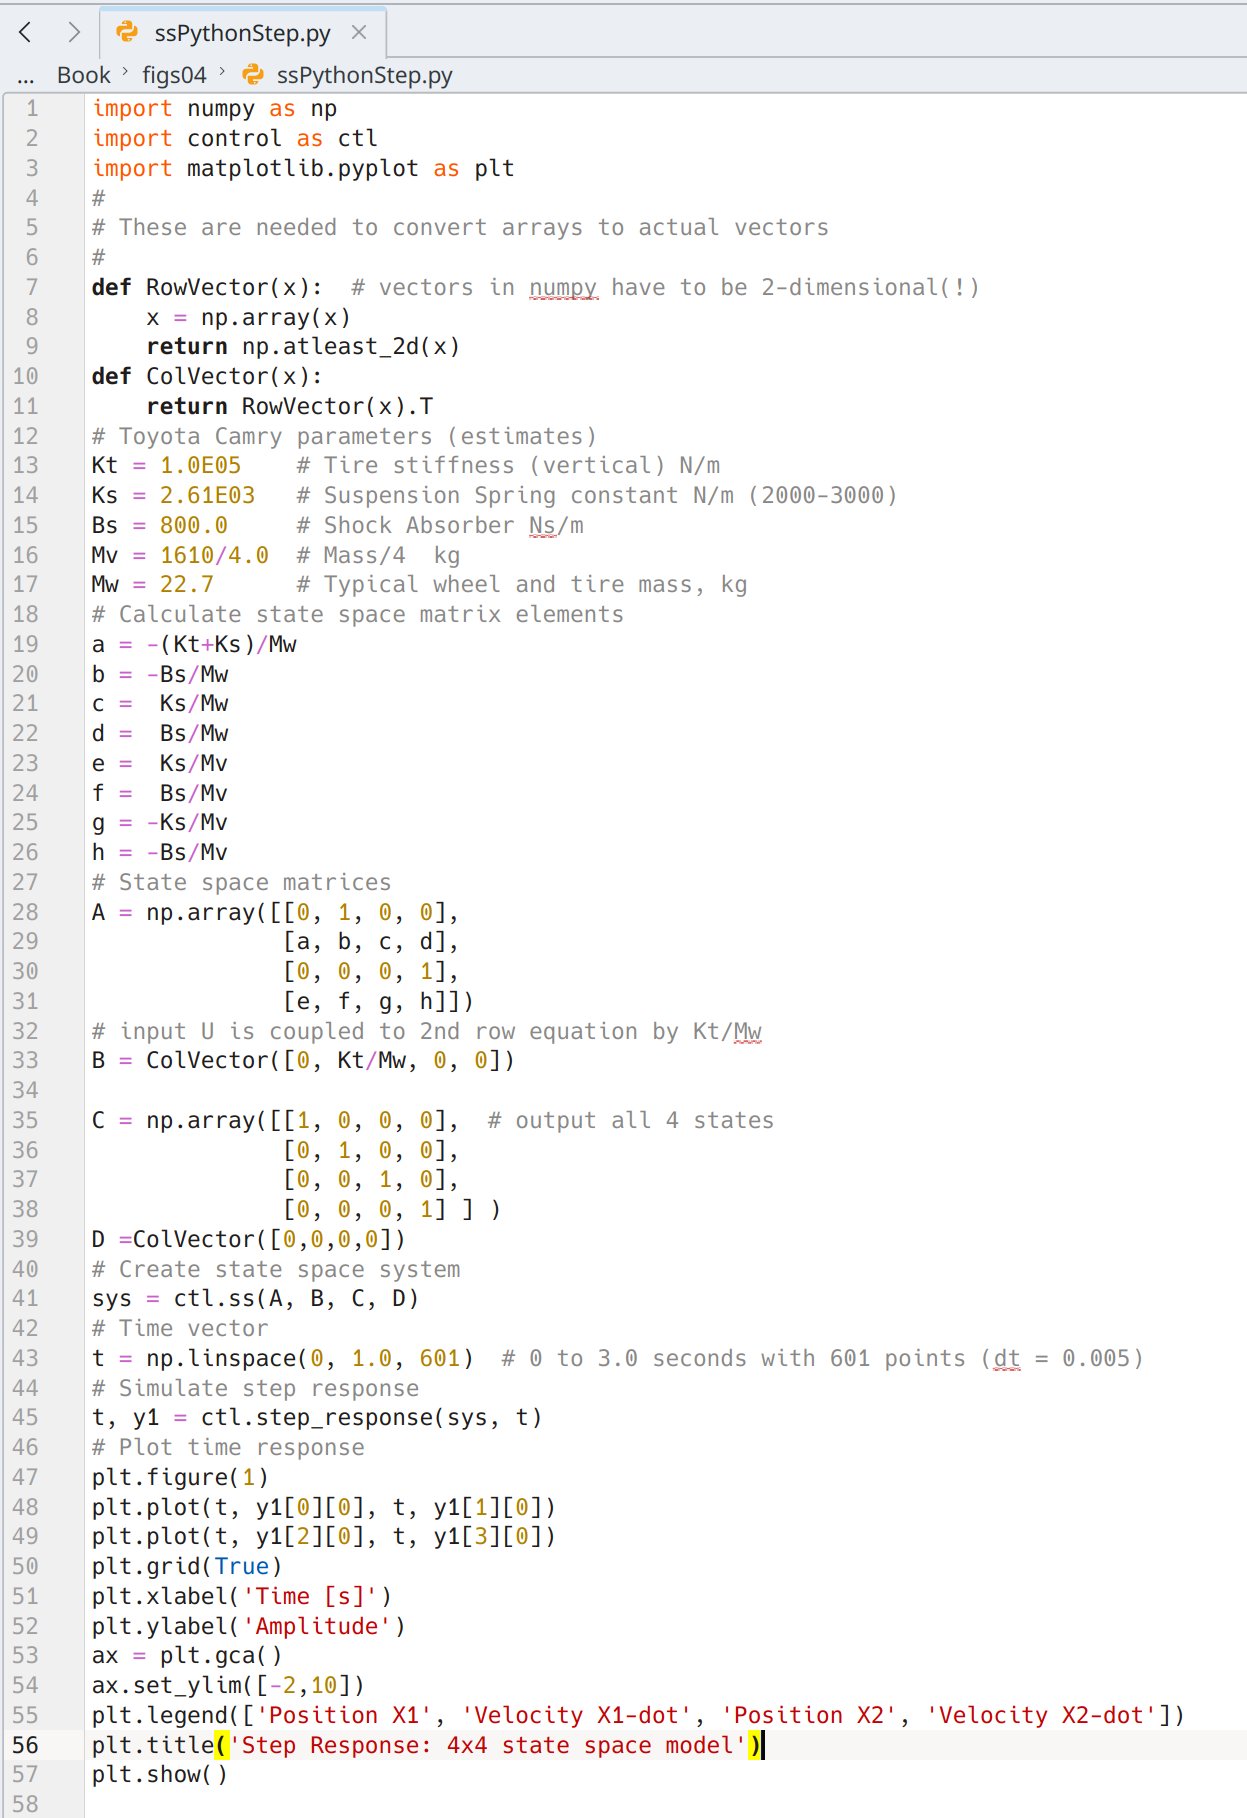
\includegraphics[width=3.5in]{figs08/python_ss_stepcode.png}
% \end{center}


In lines 7 to 11 we define our helper functions to make it easier to set up ``official"
row and column vectors in numpy.

In lines 13 to 17 we enter mechanical parameters for our car suspension.

With reference to the derived state space equation, in lines 19-26 we set
up the matrix elements, and in lines 28-39 we define the $A,B,C,D$ of the
state space equations
\[
\dot{x} = Ax+Bu
\]
\[
y = Cx + Du
\]

Recall that $x_1$ is not a 'state' but rather an input so our state vector is:

\[
x = [x_2,\dot{x_2},x_3,\dot{x}_3]^T
\]

Line 41 creates a {\tt control.StateSpace} class instance from our four matrices.

In lines 43 to 45 we compute the step response of our system.   Here we should be aware
that {\tt python.control} determines the number of inputs and outputs from the dimensions of
$B$ and $C$.   If $B>1$ or $C>1$, there is more than one transfer function based on the
permutations of inputs and outputs.   For our system here, $B$ has one column (line 33) so there
is just one input and $C$ is 4x4 meaning 4 outputs.

In lines 47 to 49 we plot 4 step responses based on a 4x4 $C$ matrix (line 35) which generates
an output vector containing the step responses.
\end{Example}
\begin{ExampleCont}
First we generate a conventional step response
\footnote{Using a simplified version of lines
48 and 49.}
from input (road displacement $x_1$) to car body
displacement ($x_2$)

% \begin{figure}\centering
\begin{center}
    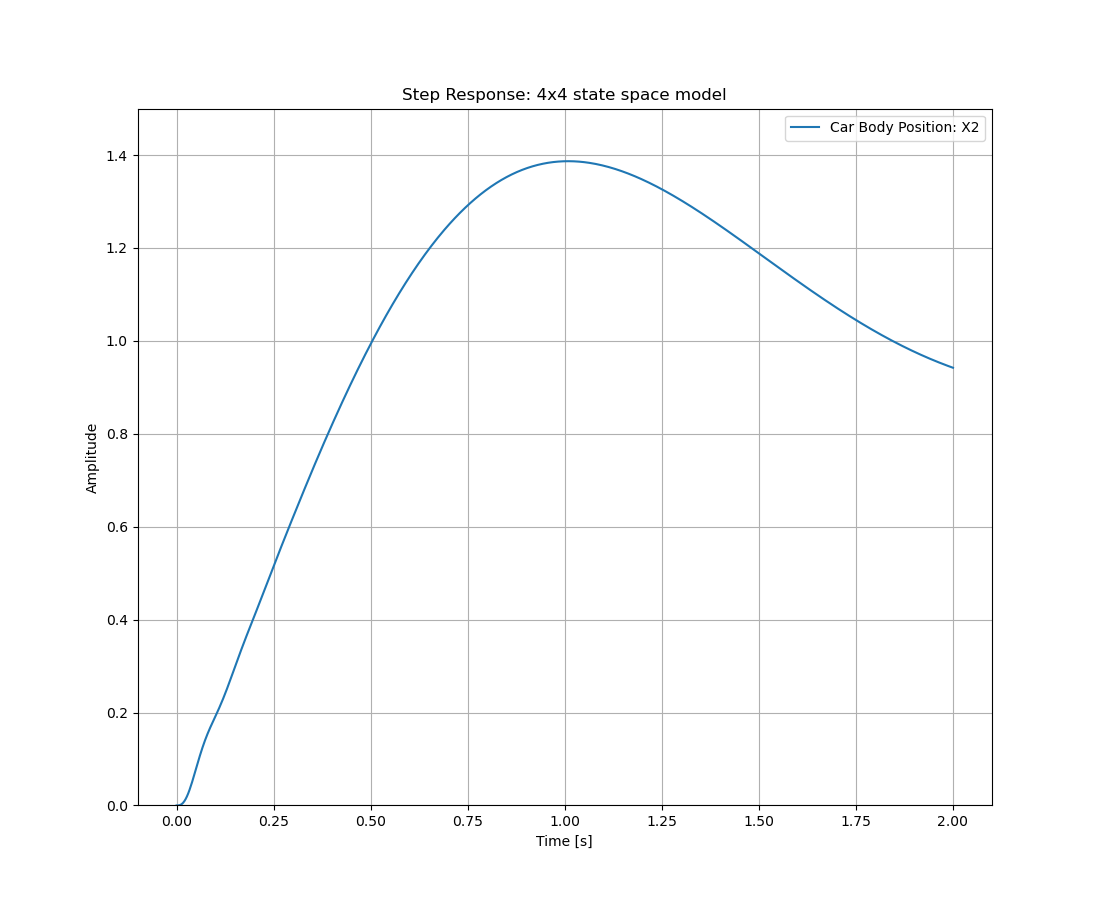
\includegraphics[width=3.5in]{figs08/singleCarBodyStep.png}

    {Step response of the car suspension system (overshoot indicates shocks probably
        worn out. Time for new ones!.)}\label{graphsuspensionstep}
\end{center}
% \end{figure}

Then, we can visualize all four state variables as they respond to a step input at $x_1$.

Let's visualize the step response in state space instead of the time domain.   We'll choose
a plane which is a subspace of state space: $[x_3, \dot{x}_3]$.   We add the following lines
to the script:

\begin{center}
    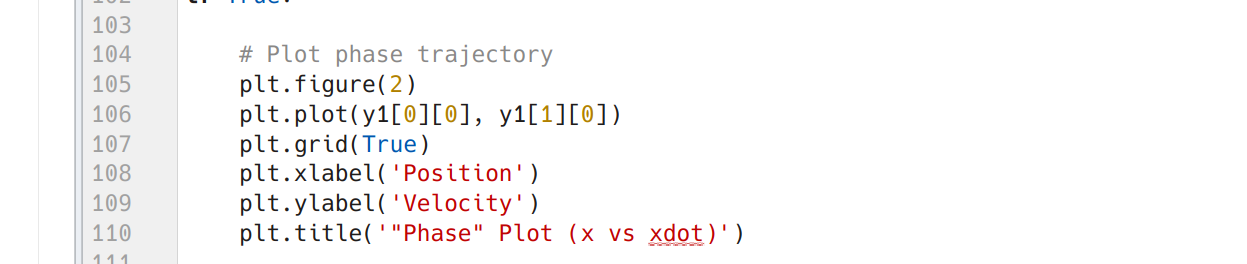
\includegraphics[width=4in]{figs08/ss_phase_addon.png}
\end{center}

Recall the second state space equation is
\[
y=Cx+Du
\]
to get the data for our subspace plot let
\[
C = \begin{bmatrix} 0,0,1,0 \\ 0,0,0,1 \end{bmatrix}
\]
Recall that $x_1$ is the road surface height, $x_2$ is the wheel axis height, and $x_3$ is the car body height.
This $C$ matrix selects out the last two elements of $X$, $Y=[x_3, \dot{x}_3]$ (line 42,43).  Then using
the same system (lines 12-41) and simulation output (line 45),
we plot the two elements of $Y$ against each other (line 106) on a new figure.
\end{ExampleCont}


\begin{listing}
\begin{minted}{python}
# System constants
K1 = 100.0
K2 = 20.0
B = 25.0
M = 100.0
# matrix elements
a = -(K1+K2)/M
b = -B/M
#  Set up A matrix
A = np.matrix([[0, 1],
[a, b]])
# Set up B matrix
# B = ColVector([0, 1/M])
B = np.matrix([[0, 0],
[0, 1/M]] )
# The input U is generated automatically as needed by ctl.step_response etc.
# output is a linear combination of x, xdot so
C = np.matrix([[2.0, 0.7],  # generate two outputs
[0,   0.0]])
# The input does not contribute directly to  output so
D = np.matrix([[0.0, 0.0],
[0.0, 0.0]])
# D = ColVector([0,0])
sys = ctl.ss(A,B,C,D)
t = np.linspace(0, 100, 601)  # 0 to 3.0 seconds with 601 points (dt = 0.005)
# Simulate step responses from every input to every output: 2x2=4 responses
stepResponseData = ctl.step_response(sys, t) # note py.ctl generates its own input
t = stepResponseData.time
y1 = stepResponseData.outputs
# Plot time response
plt.figure(1)
#
input_row = 1
output_row =0
# plt.plot(t, y1[input_row][output_row]) #
plt.plot(t, y1[output_row][input_row]) #
# Just output X_2 (body motion)
# plt.plot(t, y1[2][0])

plt.grid(True)
plt.xlabel('Time [s]')
plt.ylabel('Amplitude')
ax = plt.gca()
# ax.set_ylim([0, 0.2])
plt.legend(['Position X', 'Velocity X-dot'])
plt.title('x(t), x_dot(t) Step Responses: 2x2 state space model')
plt.show()
    \end{minted}
    \caption{{\tt python.control} State Space setup for the Auto suspension system example.}
    \label{lst:4x4ssSetup}
\end{listing}

\begin{ExampleCont}

    % \begin{figure}\centering
\begin{center}
    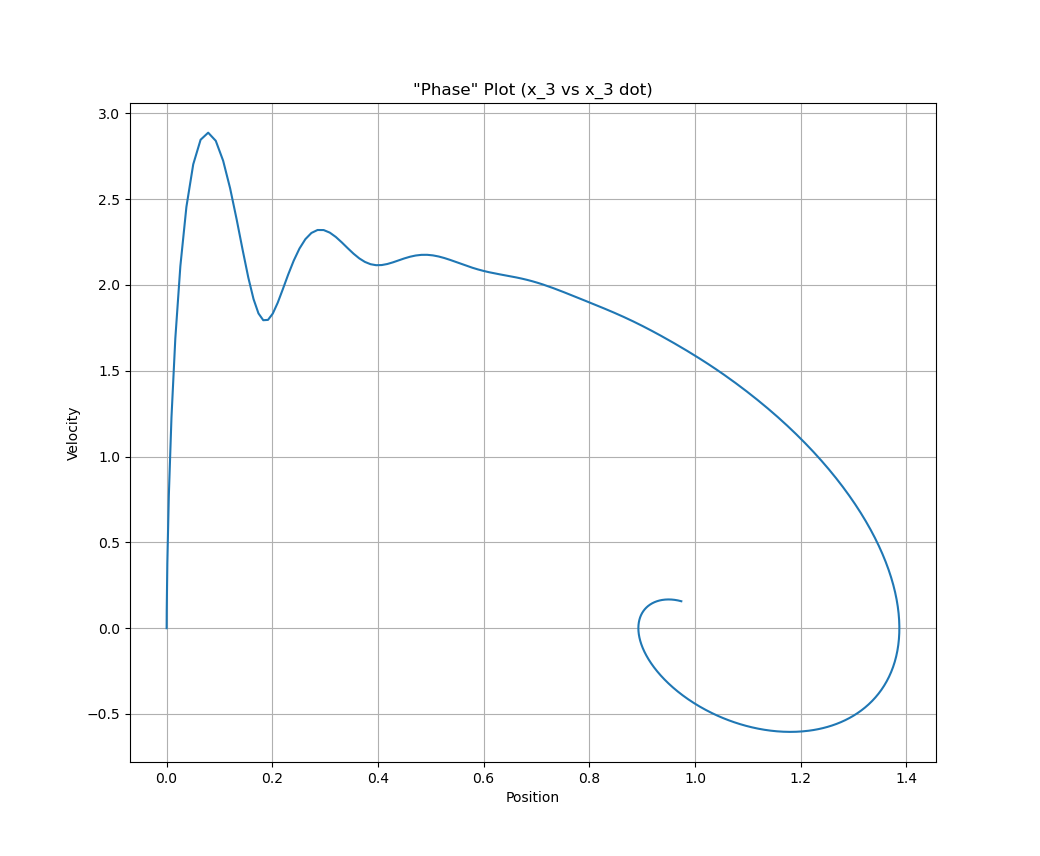
\includegraphics[width=3.5in]{figs08/py_phase_plot.png}

     {Step response of the car suspension system in state space.  Horizontal axis is $x_3$, the position of the car body, and vertical axis is $\dot{x}_3$, the velocity of the body's vertical travel.}\label{graphstatespacespiral}
\end{center}

The result  plots the body position, ($x_3$, horizontal axis) vs. body vertical velocity ($\dot{x}_3$, vertical axis).  The system trajectory starts at ($x_3=0, \quad \dot{x}_3=0$) followed by a sharp initial transient to high positive (upward)
velocity followed by an interesting spiral to the final point ($x_3=1, \quad\dot{x}_3=0$).
The $x_3(t)$ data is the same as our initial step response of this example,
and the $\dot{x}$ data is its time derivative.
Time is not explicitly shown but the spiral indicates the roughly 40\%
overshoot in the step
response and most of its convergence to the steady state position value (1.0).

Using the state space representation we can really put the dynamic response under the microscope because the $C$ matrix let's us look at all 4 state variables after a step
input. For
\[ C = \begin{bmatrix} 1, 0, 0, 0 \\ 0, 1, 0, 0 \\ 0, 0, 1, 0 \\ 0, 0, 0, 1\end{bmatrix}
\]
We see the 4 step responses of all the state variables.

\end{ExampleCont}
\begin{ExampleCont}

% \begin{figure}\centering
\begin{center}    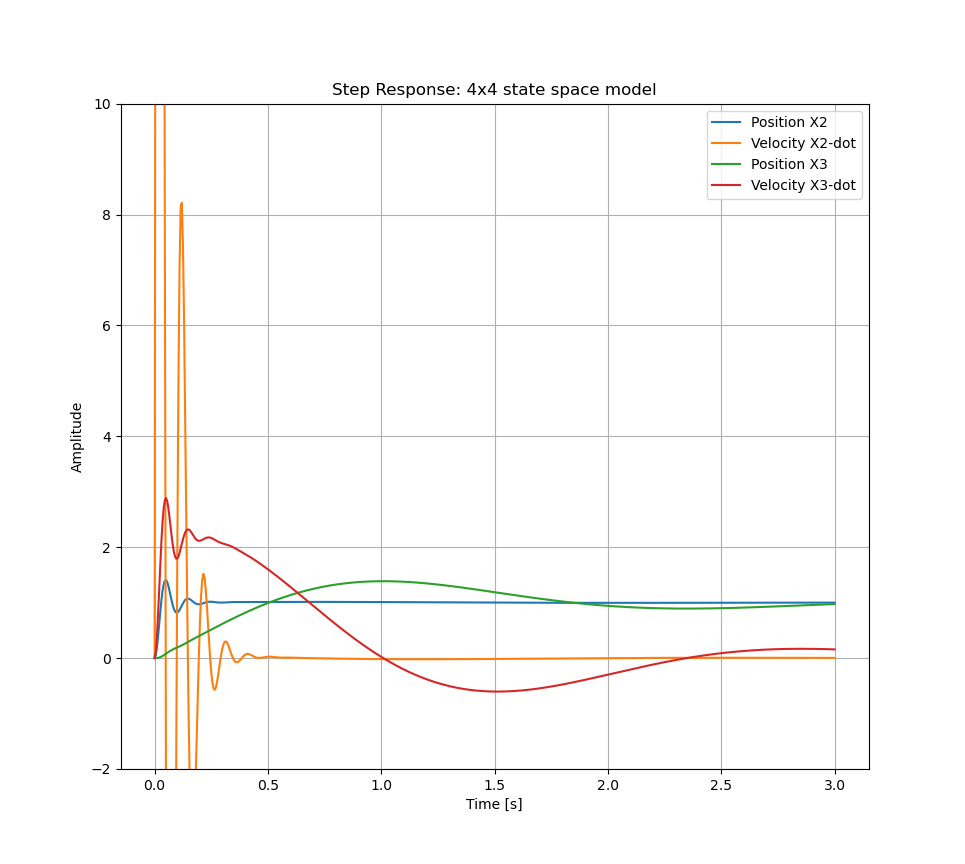
\includegraphics[width=3.5in]{figs08/all4StepResponsesCarBody.png}

    {Step response of all four states of the car suspension system from the state space model. We see the car body step response (above) is now in green (because it is the 3rd plot now).  Note change of vertical scale. }
\end{center}

\end{ExampleCont}


\subsubsection{Converting Transfer Functions to State Space and Back}

Python control has functions to easily convert back and forth between transfer functions and state space system descriptions.   For example, suppose we have the transfer function:
\[
\frac{s+2}{s^2+20s+96}
\]
we can easily use python's {\tt tf2ss(sys)} function
to convert this to a state space representation as in Listing \ref{lst:tf2ss}:



\begin{listing}
    \begin{minted}{python}
import numpy as np
import control as ctl
import matplotlib.pyplot as plt

s = ctl.TransferFunction.s
tf1 = (s+2)/(s**2+20*s+96)
ssys = ctl.tf2ss(tf1)

print(ssys)

# outputs:
#
# <StateSpace>: sys[10]
# Inputs (1): ['u[0]']
# Outputs (1): ['y[0]']
# States (2): ['x[0]', 'x[1]']
#
# A = [[-2.00000000e+01  9.60000000e+00]
#     [-1.00000000e+01 -3.88578059e-16]]
#
# B = [[1.]
#     [0.]]
#
# C = [[ 1.  -0.2]]
#
# D = [[0.]]
\end{minted}
\caption{Conversion between transfer function and state space forms (with output as comments).}
\label{lst:ss2tf}
\end{listing}



%
% \begin{center}
%     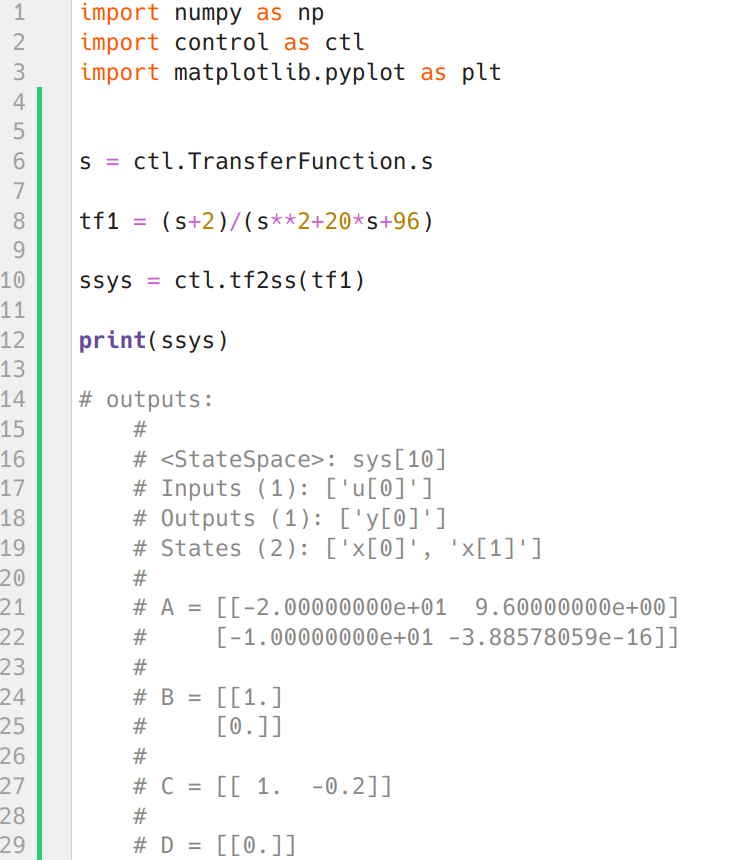
\includegraphics[width=3.5in]{figs08/Y13M75.png}
% \end{center}

Python.control returns a linear system object which contains all four matrices $A,B,C,D$.
In the computation above, the matrices $A \dots D$ are not necessarily the same as those you would
derive using the system EOMs.   However they describe an equivalent dynamical system.  It turns
out there are many SS representations for each transfer function or dynamical system.
A full treatment of this issue requires a course in modern control theory, but a few interesting
observations are worth noting.

The eigenvalues of the system matrix $A$, are the same as the poles of the transfer function.
In the example above,

\[
\frac{s+2}{s^2+20s+96} = \frac{s+2}{(s+8)(s+12)}
\]
has poles $s=\{-8,-12\}$.    The function to compute eigenvalues in python is {\tt np.linalg.eig()}.  Using
it on the matrix $A$ computed above gives $[-8, -12]$ as expected from the poles.
